\chapter{Edge Effects in the Temporal Analysis of Morphological Characteristics}\thumbforchapter
% \chaptermark{The phylotypic stage is undefined}
\chapterauthor{Maarten van der Sande, Simon J. van Heeringen}
\newpage

In 2003 Olaf R. P. Bininda-Emonds, Jonathan E. Jeffery, and and Michael K. Richardson wrote a highly critical research paper about the hourglass model and the phylotypic stage, with the title \say{\textit{Inverting the hourglass: quantitative evidence against the phylotypic stage in vertebrate development}}\cite{OlafRP2003}. Their article starts with a critique of the lack of a definition of the hourglass model and its related phylotypic stage. They then compare the timings of morphological features across different vertebrates and find an inverse hourglass-like pattern with the most variation during mid-development. Based on their analysis they argue for the existence of an inverse hourglass of conservation and conclude that there is no evidence for the hourglass model. In \textbf{Chapter 4} we discuss the need for appropriate controls and careful interpretation of comparative temporal analyses. By simulating data, we show that the methodology that Bininda-Emonds \textit{et al.} use is vulnerable to edge effects, and already produces an inverse hourglass with time-series of constant temporal variation.

Bininda-Emonds \textit{et al.} compare the rank of 116 morphological timings of developmental characteristics of 14 mammals and two amniotes with each other. This results in a table of 16 columns representing the species, and 116 rows, with each row consisting of integers in the range 1-116. These numbers represent the ranks of the timing of events within each species, which allows for the comparison of the relative timing between species. They then visualize two patterns based on these tables to estimate temporal conservation. For the first pattern, they visualize the mean rank of each morphological feature on the x-axis, and the standard error of each feature on the y-axis (Fig. \ref{fig:inverting_inversehourglass}A). This pattern exhibits a clear trend with a low standard error for features appearing early or late in development, and a high standard error for features that appear in mid-development. The authors note that this pattern could be caused by edge effects, and alternatively propose a second method that should not be vulnerable to edge effects. In this visualization, they calculate the phenotypic divergence of a group of features (PD) and visualize that against the mean rank of the group (Fig. \ref{fig:inverting_inversehourglass}B). The PD is an estimation of the diversity among species. Their visualization shows a clear curve with the highest PD during mid-development and the lowest divergence early and late during development. Both these results are in direct contradiction with the hourglass model, which caused Bininda-Emonds \textit{et al.} to argue in favor of the inverse hourglass model between mammals.

To test the claim of Bininda-Emonds \textit{et al.} that the methodology is not vulnerable to edge effects, we generated 16 identical time series consisting of the numbers 1 to 116 in order. We added Gaussian noise to these numbers with a standard deviation of 14.5 (or 1/8\textsuperscript{th} of the time series). We then calculated the ranks per time series and ordered the features based on the average rank across species. The result is that we have 16 time series of 116 ranked features with no temporal pattern of stronger conservation at specific time points. We then apply the same methodology as Bininda-Emonds \textit{et al.} and get nearly identical results (Fig. \ref{fig:inverting_inversehourglass}C-D). Despite the authors' claim that the PD visualization is not sensitive to edge effects, both the PD, and mean-standard error patterns can be fully explained by the edge effects of simulated data with no specific temporal conservation. This is caused by the effect that the most extreme timings (earliest and latest characteristics) have the smallest odds of changing their rank because an even more extreme timing does not change the ranking. As such, any set of conserved characteristics between species, with a constant level of temporal conservation, will show an inverse hourglass with these methods. Even though Bininda-Emonds \textit{et al.} are rightfully frustrated by the lack of a definition of the phylotypic stage and quantitative proof for it, we see no evidence for their claim of an inverse hourglass based on morphological characteristics. Consequently, this analysis is consistent with our recommendations in
\textbf{Chapter 4} for implementing proper controls in comparative research.

\begin{figure} [H]
    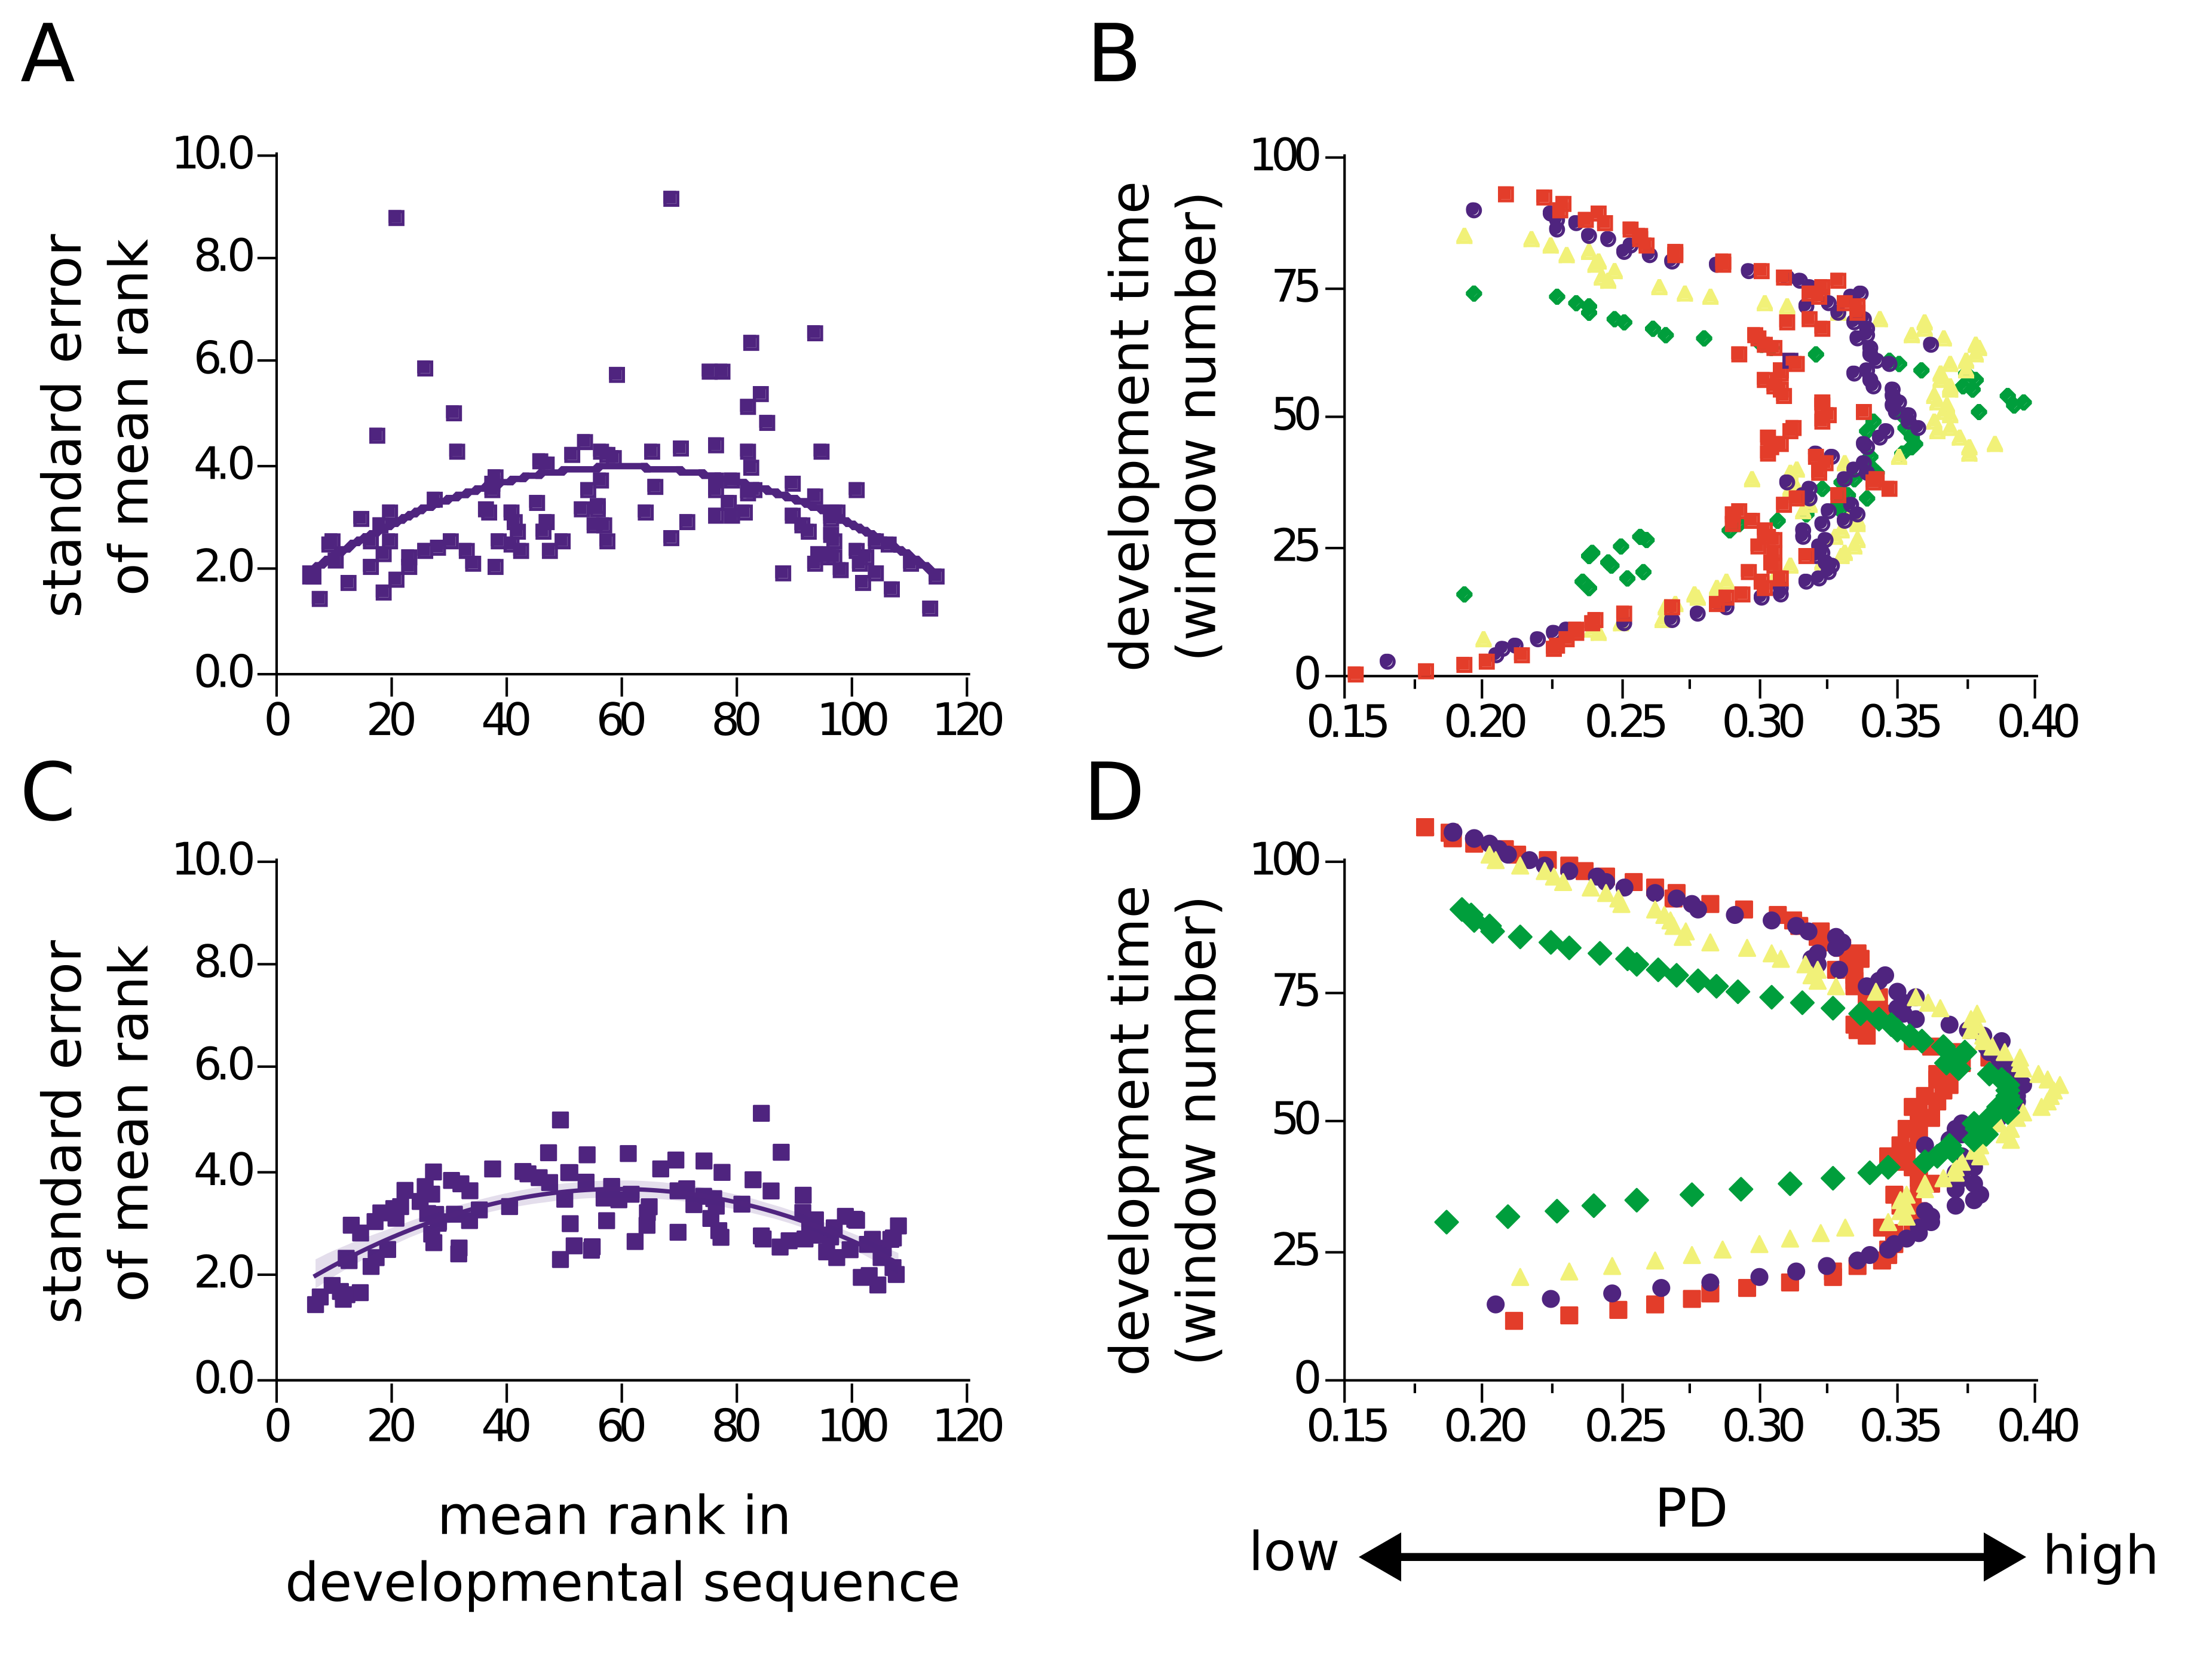
\includegraphics[width=\linewidth]{ch.inverthourglass/imgs/inverting.png}
    \caption{\textbf{Simulations without any temporal conservation pattern capture the same dynamics as data based on real timings of morphological characteristics.} \textbf{(A)} Figure taken directly from Bininda-Emonds \textit{et al.}\cite{OlafRP2003} which shows the standard error of the mean rank of a developmental event versus the mean rank based on real data. \textbf{(B)} Figure taken directly from Bininda-Emonds \textit{et al.}\cite{OlafRP2003} which shows overlapping windows (\textit{i.e.} composed of events of ranks 1–5, 2–6, 3–7, ...) with durations of one-fifth (red squares), one-quarter (blue circles), one-third (yellow triangles) or one-half (green diamonds) of the length of the developmental time span examined based on real data. \textbf{(C-D)} are based on simulated data with no specific temporal conservation, and show the same patterns as the real data of panels A and B. }
    \label{fig:inverting_inversehourglass}
\end{figure}

\newpage

\section{Methods}

\subsection{Phenotypic divergence}

The PD is calculated identical to Bininda-Emonds \textit{et al.},  in sliding windows of 1/5, 1/4, 1/3, and 1/2 of the total time series by the original authors to avoid artefacts arising from a single subjective placement of an event. 

\begin{align*}\label{eq:phenotypicdivergence}
    \text{events} &= \{1^{st}\text{ somite pair}, 4^{th}\text{ somite pair}, ...,\text{ neural fold fusing}\} \\ 
    PD_{\text{event}} &= 1 - \frac{|n_{\text{present}} - n_{\text{absent}}|}{n_{\text{present}} + n_{\text{absent}}} \\
    PD &= \frac{1}{|\text{events}|} \sum_{\text{event}}^{\text{events}} PD_{\text{event}}
\end{align*}

\subsection{Simulated data}

The simulation of the data was conducted using Python 3.10, leveraging libraries such as numpy and pandas for data manipulation, and matplotlib and seaborn for visualization.

\begin{lstlisting}[language=Python]
import pandas as pd
import numpy as np
import matplotlib.pyplot as plt
import seaborn as sns

fig, axs = plt.subplots(ncols=2)

def make_random_data(n=10, t=100):
    # make n identical time series of t long
    xs = pd.DataFrame([np.arange(0, t) for _ in range(n)])
    
    # add gaussian noise
    xs +=  np.random.normal(0, t/8, xs.shape) 
    
    # convert to ranks per time series
    xs = xs.rank(axis=1)
    
    # sort the features based on average occurrence
    xs = xs[xs.mean().sort_values().index]
    
    return xs

xs = pd.DataFrame(make_random_data(n=16, t=116))
sns.regplot(x=xs.mean(axis=0), 
            y=xs.sem(axis=0),
            order=2,
            color="#4f247fff", 
            marker="s",
            scatter_kws={"s": 60, "alpha":1},
            ax=axs[0]
)
axs[0].axis(xmin=0.0,xmax=120, ymin=0, ymax=10)

def phenotypic_diversity(xs):
    PD = []
    for i in range(1, 116):
        n_present = (i == xs).sum().sum()
        n_absent = xs.shape[0] - n_present

        PD_e = 1 - np.abs((n_present - n_absent) / (n_present + n_absent))
        PD.append(PD_e)
    return np.mean(PD)

colors = ["#e33d2a", "#4f247f", "#f1f178", "#009e3c"]
markers = ["s", "o", "^", "D"]
stepsizes = [xs.shape[1]//5, xs.shape[1]//4, xs.shape[1]//3, xs.shape[1]//2]

for stepsize, color, marker in zip(stepsizes, colors, markers):
    PDs = [phenotypic_diversity(xs.iloc[:, i:i+stepsize]) for i in range(0, xs.shape[1] - stepsize)]
    windows = [x + (xs.shape[1] - len(PDs)) // 2 for x in range(len(PDs))]
    axs[1].scatter(PDs, windows, c=color, s=60, marker=marker)
axs[1].axis(xmin=0.15,xmax=0.45, ymin=0, ymax=100)
\end{lstlisting}

